\section{Theorie}
\label{sec:Theorie}

\subsection{Einletung}
In diesem Versuch wird Licht am Spalt gebeugt, dieser weißt einen kleineren Durchmesser als das klassiche
Strahlbündel auf. Bei der Beugung entstehen Phänomene die den Gesetzen der geometrischen Optik wiedrsprechen.
Ein Beugungsbild entsteht, welches Gegenstand dieses Experimentes ist.

\subsection{Beugung}
Es existieren zwei Beugungsarten, zum einen die Fresnel-Beugung: hierbei wird angenommen, dass eine
Quelle eine endliche Entfernung vom Detektor hat, somit werden alle Strahlen die im Punkt P inteferieren
unter unterschiedlichen Winkeln gebeugt. Im Gegensatz dazu steht die Frauenhofer-Beugung, hier ist
die Quelle im Unendlichen und damit werden alle Strahlen unter dem gleichen Winkel gebeugt, wie in Abbildung
\ref{fig:BA} zu sehen.
 \begin{figure}
  \centering
  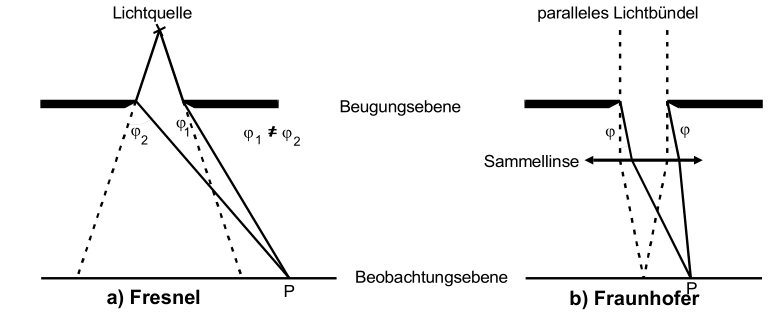
\includegraphics[width=0.6\textwidth]{BA.PNG}
  \caption{Beide Beugungsarten, hier zeigen die gestrichelten Linien den Verlauf nach der Geometrischen Optik an.}
  \label{fig:BA}
\end{figure}
Da die Frauenhofer-Beugung mathematisch einfacher zu handhaben ist, wird diese mittels Laser realisiert.
Eine weitere Vereinfachung ist die Länge des Spaltes größer gegenüber seiner Breite, damit entsteht nur
in einer Dimension Beugung.
Die Beugungserscheinungen könnnen durch die Kombination aus Huygenschen Prinzip und dem Interferenzprinzip nach Fresnel beschriebeen werden.
Ersteres besagt, dass jeder Punkt einer Wellenfront Ausgangspunkt für eine neue Elementarwelle ist.
Das Interferenzprinzip sagt aus, dass es zwischen Wellen zur Interferenz kommt und somit eine neue Wellenfront
entsteht, welche als Einhüllende bezeichnet wird.
\subsection{Einzelspalt}
Es werden zwei einfallende Strahlenbündel betrachtet, diese gehen von zwei verschiedenen Punkten im Abstand x vom
Spalt aus. Die Strahlenbündel haben wegen des Gangunterschieds eine Phasendifferen von:
\begin{align}
\delta = \frac{2\pi x \sin\phi}{\lambda}.
\end{align}
Nach weiteren Betrachtungen und der Intergration über die Spaltbreite $b$ ergibt sich:
\begin{align}
B(z,t,\phi)=A_0 e^{\left(i\left(\omega t\cdot\frac{2\pi z}{\lambda}\right)\right)}\cdot e^{\left(\frac{\pi i b\sin\phi}{\lambda}\right)}\cdot\frac{\lambda}{\pi\sin\phi}\sin\left(\frac{\pi b \sin\phi}{\lambda}\right).
\end{align}
Für experimentelle Betrachtungen sind die beiden e-Funktionen irrelevant, damit vereinfacht sich die Gleichung zu:
\begin{align}
B(\phi)=A_0 b \frac{sin \eta}{\eta} \ \ \ \ \text{mit} \ \ \ \eta=\frac{\pi b \sin \phi}{\lambda}.
\end{align}
Die Amplitude einer Lichtquelle ist nicht direkt messbar, deshalb wird auf die Intensität zurückgegriffen:
\begin{align}
I(\phi)\propto B(\phi)^2 = A_0^2 b^2\left(\frac{\lambda}{\pi b \sin\phi}\right)^2\cdot\sin^2\left(\frac{\pi b \sin\phi}{\lambda}\right).
\end{align}
\subsection{Doppelspalt}
Für einen Doppelspalt gelten analoge Betrachtungen, da dieser sich aus der Überlagerung zweier Einzelspalte
mit Breite $b$ und Abstand $s$ zusammensetzt. Es gilt:
\begin{align}
I(\phi) \propto B(\phi)^2 = 4\cos^2\left(\frac{\pi s sin\phi}{\lambda}\right)\cdot\left(\frac{\lambda}{\pi s \sin\phi}\right)^2\cdot\sin^2\left(\frac{\pi b \sin\phi}{\lambda}\right.
\end{align}
Diese Intensitätsverteilung enthält zusätzlich $cos^2$-Terme.
\subsection{Fourier-Transformierte}
Die Amplitudenverteilung lässt sich auch auf allgemeine Weise Berechnen, dazu lässt sich $B(\phi)$ als
Fourier-Transformierte der Amplitudenverteilung der einfallenden Welle in der Beugungsebene darstellen.
Allgemein gilt für eine Fourier-Transformation einer Funktion f(x):
\begin{align}
g(\xi)= \int_-\infty^\infty f(x) \cdot e^{ix\xi} \mathrm{d}x.
\end{align}
Am Spalt gilt $f(x)=A_0$, durch  Einsetzen und anschließendes Anwenden der Eulerschen Formle ergibt sich:
\begin{align}
g(\xi)=\frac{2A_0}{\xi} e^{\frac{i\xi b}{2}}\sin\left(\frac{\xi b}{2}\right).
\end{align}
Für $\xi$ kann $\xi=\frac{2\pi\sin\phi}{\lambda}$ eingesetzt werden, so lässt sich erkennen, dass das Huygensche Prinzip
durch die Fourier-Transformierte mathematisch beschrieben werden kann.
